% !TEX root = _individual/introduction.tex

%%%%%%%%%%%%%%%%%%%%%%%%%%%%%%%%%%%%%%%%%%%%%%%%%%%%%%%%%%%%%%%%%%%%%%%%%%%%%%%%
\chapter{Introduction}\label{chap:introduction}
%%%%%%%%%%%%%%%%%%%%%%%%%%%%%%%%%%%%%%%%%%%%%%%%%%%%%%%%%%%%%%%%%%%%%%%%%%%%%%%%
This thesis extends an anisotropic diffusion (AD) approximation to
infinite-medium, steady-state particle transport \cite{Mor2007,Lar2009c},
formulating a more general theory that applies to
time-dependent nonlinear particle transport with arbitrary problem boundaries.
Our motivation is to formulate and test an approximation to thermal radiative
transfer (TRT) that is more accurate than diffusion yet much less expensive
than a time-dependent transport calculation.

The past fifty years in which computers have been used to simulate radiative
transfer problems \cite{Cam1964,Cam1969} have seen unbelievable
advancements in computer technology.
Yet even today, with the need for increasingly accurate simulation of
increasingly
large and complex problems, computational power is still a limiting factor.
This is especially true in the burgeoning field of Uncertainty Quantification
(UQ), in which large numbers of computer simulations are needed to gauge the
accuracy in the solution of a single problem.

It is one such problem in particular that inspired this work. The Center for
RAdiative Shock Hydrodynamics (CRASH) program \cite{Crash2010} has the goal of
computationally predicting the behavior of a laser-driven shock in a
xenon-filled tube and providing ``error bars'' for that prediction. The accurate
simulation of energy traveling down a hollow pipe is critical to modeling that
problem, and several of the numerical test problems in this thesis are based
on it.

Existing approximations to TRT, represented qualitatively in
Fig.~\ref{fig:fidelity}, are essentially either very accurate or very fast. On
the one hand are Fleck and Cummings' Implicit Monte Carlo (IMC) method
\cite{Fle1971} and the discrete ordinates (\SN) method \cite{Ada1998a}, which
require both significant time and large amounts of computer memory. On the
other hand is, for example, the flux-limited diffusion (FLD) method
\cite{Ols2000}, which sacrifices accuracy for speed. By developing a
time-dependent anisotropic diffusion approximation, we hope to provide a middle
ground that exchanges some minor amount of speed for a significant increase in
accuracy. The AD method could then be applied to the CRASH project to yield
realistic results in a realistic amount of time.

\begin{figure}[htb]
  \centering
  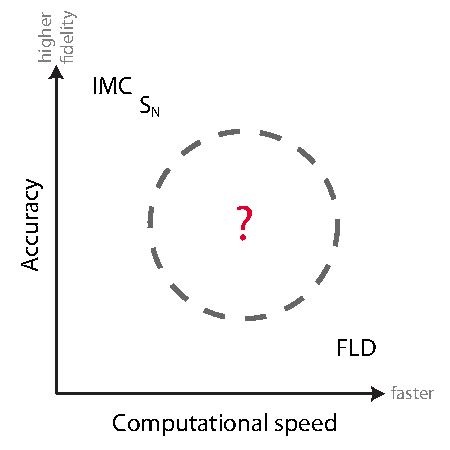
\includegraphics[width=3in]{fidelity}
  \caption{Figurative representation of existing TRT methods, showing the
  trade-off between accuracy and speed.}
  \label{fig:fidelity}
\end{figure}



\section{Synopsis}
The remainder of this thesis is organized into the following chapters.

\chaptersynopsis{chap:trtBackground}
The assertions about the difficulty of computational modelling of thermal
radiative transfer are bolstered by presenting the equations themselves. We give
a brief overview of existing approximations to the TRT regime and discuss how
those approximations are used in our work. Particular emphasis is given to the
semi-implicit treatment, which allows the nonlinear problem to be approximated
by a system of linear equations.

\chaptersynopsis{chap:adDerivation}
With the transport equation in hand, we derive a new approximation to radiation
transport, anisotropic diffusion. The derivation accounts for both the time
dependence and boundary conditions. We then discuss some of the properties of
the AD method and make predictions for its range of applicability.

\chaptersynopsis{chap:aponeDerivation}
The derivation for the time-dependent AD equations assumed that the solution
changes very slowly in time, which can be a poor approximation when applied to
TRT that leads to the nonphysical transfer of energy faster than the speed of
light. This chapter addresses that shortcoming in two very different ways. The
first is to apply the physically motivated but \emph{ad hoc} method of flux
limiting to the AD formulation. The second is to modify the ansatz used in
deriving the anisotropic diffusion equations, leading to the \APone\ method.

\chaptersynopsis{chap:implementation}
The leakage terms for anisotropic diffusion are more complex than standard
diffusion: rather than a scalar diffusion coefficient, AD has a diffusion
tensor. This necessitates unusual discretization schemes in all but the simplest
of problems. We derive new discretization schemes for Cartesian \xy\ geometry
that can account for the transverse leakage induced by the anisotropic diffusion
tensor.

\chaptersynopsis{chap:flatland}
As mentioned earlier, the ``flatland'' geometry has recently proven to be a
valuable test bed for new transport methods because of its smaller phase space
and correspondingly easier solution. This chapter gives a thorough overview of
the differences between flatland and true 3D geometries, with a focus on
implementing flatland solvers. We also explore diffusion in flatland, not only
deriving the prior result that the diffusion coefficient is different but also
formulating correct diffusion boundary conditions. Finally, we present the AD
equations in flatland geometry.

\chaptersynopsis{chap:simpleNumericalResults}
Before applying the anisotropic approximations to full nonlinear transport in
multi-dimensional geometries, it is important that we test individual components
of the derivation. We detail several steady-state problems that test the
discretization schemes, flatland diffusion boundary conditions, and anisotropic
diffusion boundary conditions.

\chaptersynopsis{chap:trtNumericalResults}
Finally, we test the applicability of the anisotropic methods to the nonlinear
TRT equations. To begin, we look at a few simple 1-D test problems, where the
anisotropic methods merely ``smear'' the diffusion coefficients spatially. Then
we move to more complicated flatland problems that simulate radiation flow
through an optically thin channel, most applicable to the CRASH program.
Additionally, we apply the AD method to some difficult 2-D problems in the
literature that feature optically thick obstacles rather than optically thin
streaming channels.

\chaptersynopsis{chap:conclusion}
The final chapter summarizes the results of the theory developed in this work
and its application to TRT problems. We discuss possible improvements to the new
methods and other future work.

